\documentclass[dvisvgm,tikz]{standalone}
\usepackage{tikz}
\usetikzlibrary{positioning,decorations.pathreplacing,calc}
\begin{document}
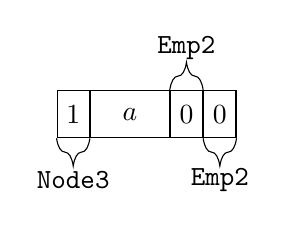
\begin{tikzpicture}
  \node[rectangle,draw,minimum height=0.6cm] (first) {$1$};
  \node[rectangle,draw,minimum height=0.6cm,minimum width=1cm,right=0cm of first] (second) {$a$};
  \node[rectangle,draw,minimum height=0.6cm, right=0cm of second] (third) {$0$};
  \node[rectangle,draw,minimum height=0.6cm, right=0cm of third] (fourth) {$0$};
  \draw[decorate,decoration= {brace,mirror,amplitude=10pt}] (first.south west) -- (first.south east) node [midway,yshift=-15pt] {\texttt{Node3}};
  \draw[decorate,decoration= {brace,amplitude=10pt}] (third.north west) -- (third.north east) node [midway,yshift=15pt] {\texttt{Emp2}};
  \draw[decorate,decoration= {brace,mirror,amplitude=10pt}] (fourth.south west) -- (fourth.south east) node [midway,yshift=-15pt] {\texttt{Emp2}};
\end{tikzpicture}
\end{document}

